
\section{Experiment Details and Full Results}
\label{sec:experiment-details}

This section contains full experimental procedures and extended results and citations for our experimental evaluation in \cref{sec:experiments}.
\cref{sec:experiment-details-benchmarking} corresponds to benchmarking results in \cref{sec:experiments-benchmark},
\cref{sec:experiment-details-lrd} corresponds to LRD experiments (LRA and Speech Commands) in \cref{sec:experiments-lrd},
and \cref{sec:experiment-details-general} corresponds to the general sequence modeling experiments (generation, image classification, forecasting) in \cref{sec:experiments-general}.

\subsection{Benchmarking}
\label{sec:experiment-details-benchmarking}

Benchmarking results from \cref{tab:ssm-benchmark} and \cref{tab:lra-benchmark} were tested on a single A100 GPU.

\paragraph{Benchmarks against LSSL}

For a given dimension \( H \), a single LSSL or \methodabbrv{} layer was constructed with \( H \) hidden features.
For LSSL, the state size \( N \) was set to \( H \) as done in \citep{gu2021lssl}.
For \methodabbrv{}, the state size \( N \) was set to parameter-match the LSSL, which was a state size of \( \frac{N}{4} \) due to differences in the parameterization.
\cref{tab:ssm-benchmark} benchmarks a single forward+backward pass of a single layer.

\paragraph{Benchmarks against Efficient Transformers}
Following \citep{tay2021long}, the Transformer models had 4 layers, hidden dimension \( 256 \) with \( 4 \) heads, query/key/value projection dimension \( 128 \), and batch size \( 32 \), for a total of roughly \( 600k \) parameters.
The \methodabbrv{} model was parameter tied while keeping the depth and hidden dimension constant (leading to a state size of \( N = 256 \)).

We note that the relative orderings of these methods can vary depending on the exact hyperparameter settings.

\subsection{Long-Range Dependencies}
\label{sec:experiment-details-lrd}
This section includes information for reproducing our experiments on the Long-Range Arena and Speech Commands long-range dependency tasks.

\paragraph{Long Range Arena}

\cref{tab:lra-full} contains extended results table with all 11 methods considered in \citep{tay2021long}.

\begin{table}[t]
  \small
  \caption{Full results for the Long Range Arena (LRA) benchmark for long-range dependencies in sequence models. (Top): Original Transformer variants in LRA. (Bottom): Other models reported in the literature.}
    \centering
    \begin{tabular}{@{}llllllll@{}}
        \toprule
        Model                 & \textsc{ListOps}  & \textsc{Text}     & \textsc{Retrieval} & \textsc{Image}    & \textsc{Pathfinder} & \textsc{Path-X} & \textsc{Avg}      \\
        \midrule
        Random                & 10.00             & 50.00             & 50.00              & 10.00             & 50.00               & 50.00           & 36.67             \\
        \midrule
        Transformer           & 36.37             & 64.27             & 57.46              & 42.44             & 71.40               & \xmark          & 53.66             \\
        Local Attention       & 15.82             & 52.98             & 53.39              & 41.46             & 66.63               & \xmark          & 46.71             \\
        Sparse Trans.         & 17.07             & 63.58             & 59.59              & 44.24             & 71.71               & \xmark          & 51.03             \\
        Longformer            & 35.63             & 62.85             & 56.89              & 42.22             & 69.71               & \xmark          & 52.88             \\
        Linformer             & 35.70             & 53.94             & 52.27              & 38.56             & 76.34               & \xmark          & 51.14             \\
        Reformer              & \underline{37.27} & 56.10             & 53.40              & 38.07             & 68.50               & \xmark          & 50.56             \\
        Sinkhorn Trans.       & 33.67             & 61.20             & 53.83              & 41.23             & 67.45               & \xmark          & 51.23             \\
        Synthesizer           & 36.99             & 61.68             & 54.67              & 41.61             & 69.45               & \xmark          & 52.40             \\
        BigBird               & 36.05             & 64.02             & 59.29              & 40.83             & 74.87               & \xmark          & 54.17             \\
        Linear Trans.         & 16.13             & \underline{65.90} & 53.09              & 42.34             & 75.30               & \xmark          & 50.46             \\
        Performer             & 18.01             & 65.40             & 53.82              & 42.77             & 77.05               & \xmark          & 51.18             \\
        \midrule
        FNet                  & 35.33             & 65.11             & 59.61              & 38.67             & \underline{77.80}   & \xmark          & 54.42             \\
        Nystr{\"o}mformer     & 37.15             & 65.52             & \underline{79.56}  & 41.58             & 70.94               & \xmark          & 57.46             \\
        Luna-256              & 37.25             & 64.57             & 79.29              & \underline{47.38} & 77.72               & \xmark          & \underline{59.37} \\
        \textbf{\methodabbrv} (original) & 58.35   & 76.02 & 87.09     & 87.26 & 86.05      & 88.10  & 80.48 \\
        \textbf{\methodabbrv} (updated)  & \textbf{59.60}   & \textbf{86.82} & \textbf{90.90}     & \textbf{88.65} & \textbf{94.20}      & \textbf{96.35}  & \textbf{86.09} \\
        \bottomrule
    \end{tabular}
    \label{tab:lra-full}
\end{table}

For the \methodabbrv{} model, hyperparameters for all datasets are reported in \cref{tab::best-hyperparameters}.
For all datasets, we used the AdamW optimizer with a constant learning rate schedule with decay on validation plateau.
However, the learning rate on HiPPO parameters (in particular \( \bm{\Lambda}, \bm{P}, \bm{Q}, \bm{B}, \bm{C}, \dt \)) were reduced to a maximum starting LR of \( 0.001 \), which improves stability since the HiPPO equation is crucial to performance.

The \methodabbrv{} state size was always fixed to \( N=64 \).

As \methodabbrv{} is a sequence-to-sequence model with output shape (batch, length, dimension) and LRA tasks are classification,
mean pooling along the length dimension was applied after the last layer.

We note that most of these results were trained for far longer than what was necessary to achieve SotA results (e.g., the \texttt{Image} task reaches SotA in 1 epoch).
Results often keep improving with longer training times.

\textbf{Updated results.}
The above hyperparameters describe the results reported in the original paper, shown in \cref{tab:lra-full}, which have since been improved.
See \cref{sec:reproduction}.

\textbf{Hardware.}
All models were run on single GPU.
Some tasks used an A100 GPU (notably, the Path-X experiments), which has a larger max memory of 40Gb.
To reproduce these on smaller GPUs, the batch size can be reduced or gradients can be accumulated for two batches.

\begin{table*}[!t]
  \caption{
    The values of the best hyperparameters found for classification datasets; LRA (Top) and images/speech (Bottom).
    LR is learning rate and WD is weight decay. BN and LN refer to Batch Normalization and Layer Normalization.
  }
  \label{tab::best-hyperparameters}
  \centering
  \resizebox{\textwidth}{!}{%
    \begin{tabular}{@{}llllllllllll@{}}
      \toprule
                                      & \textbf{Depth} & \textbf{Features \( H \)} & \textbf{Norm} & \textbf{Pre-norm} & {\bf Dropout} & {\bf LR} & {\bf Batch Size} & {\bf Epochs} & \textbf{WD} & \textbf{Patience} \\
      \midrule
      \textbf{ListOps}                & 6              & 128                       & BN            & False             & 0             & 0.01     & 100              & 50           & 0.01        & 5                 \\
      \textbf{Text}                   & 4              & 64                        & BN            & True              & 0             & 0.001    & 50               & 20           & 0           & 5                 \\
      \textbf{Retrieval}              & 6              & 256                       & BN            & True              & 0             & 0.002    & 64               & 20           & 0           & 20                \\
      \textbf{Image}                  & 6              & 512                       & LN            & False             & 0.2           & 0.004    & 50               & 200          & 0.01        & 20                \\
      \textbf{Pathfinder}             & 6              & 256                       & BN            & True              & 0.1           & 0.004    & 100              & 200          & 0           & 10                \\
      \textbf{Path-X}                 & 6              & 256                       & BN            & True              & 0.0           & 0.0005   & 32               & 100          & 0           & 20                \\
      \midrule
      \textbf{CIFAR-10}               & 6              & 1024                      & LN            & False             & 0.25          & 0.01     & 50               & 200          & 0.01        & 20                \\
      \midrule
      \textbf{Speech Commands (MFCC)} & 4              & 256                       & LN            & False             & 0.2           & 0.01     & 100              & 50           & 0           & 5                 \\
      \textbf{Speech Commands (Raw)}  & 6              & 128                       & BN            & True              & 0.1           & 0.01     & 20               & 150          & 0           & 10                \\
      \bottomrule
    \end{tabular}%
  }
\end{table*}


\paragraph{Speech Commands}
We provide details of sweeps run for baseline methods run by us---numbers for all others method are taken from \citet{gu2021lssl}. The best hyperparameters used for \methodabbrv{} are included in Table~\ref{tab::best-hyperparameters}.

\textit{Transformer~\citep{vaswani2017attention}} For MFCC, we swept the number of model layers $\{2, 4\}$, dropout $\{0, 0.1\}$ and learning rates $\{0.001, 0.0005\}$. We used $8$ attention heads, model dimension $128$, prenorm, positional encodings, and trained for $150$ epochs with a batch size of $100$. For Raw, the Transformer model's memory usage made training impossible.

\textit{Performer~\citep{choromanski2020rethinking}} For MFCC, we swept the number of model layers $\{2, 4\}$, dropout $\{0, 0.1\}$ and learning rates $\{0.001, 0.0005\}$. We used $8$ attention heads, model dimension $128$, prenorm, positional encodings, and trained for $150$ epochs with a batch size of $100$. For Raw, we used a model dimension of $128$, $4$ attention heads, prenorm, and a batch size of $16$. We reduced the number of model layers to $4$, so the model would fit on the single GPU. We trained for $100$ epochs with a learning rate of $0.001$ and no dropout.

\textit{ExpRNN~\citep{lezcano2019cheap}} For MFCC, we swept hidden sizes $\{256, 512\}$ and learning rates $\{0.001, 0.002, 0.0005\}$. Training was run for $200$ epochs, with a single layer model using a batch size of $100$. For Raw, we swept hidden sizes $\{32, 64\}$ and learning rates $\{0.001, 0.0005\}$ (however, ExpRNN failed to learn).

\textit{LipschitzRNN~\citep{erichson2021lipschitz}} For MFCC, we swept hidden sizes $\{256, 512\}$ and learning rates $\{0.001, 0.002, 0.0005\}$. Training was run for $150$ epochs, with a single layer model using a batch size of $100$. For Raw, we found that LipschitzRNN was too slow to train on a single GPU (requiring a full day for $1$ epoch of training alone).

\textit{WaveGAN Discriminator~\citep{Donahue2019AdversarialAS}}
The WaveGAN-D in \cref{tab:sc} is actually our improved version of the discriminator network from the recent WaveGAN model for speech~\citep{Donahue2019AdversarialAS}.
This CNN actually did not work well out-of-the-box, and we added several features to help it perform better.
The final model is highly specialized compared to our model, and includes:
\begin{itemize}%
  \item Downsampling or pooling between layers, induced by strided convolutions, that decrease the sequence length between layers.
  \item A global fully-connected output layer; thus the model only works for one input sequence length and does not work on MFCC features or the frequency-shift setting in \cref{tab:sc}.
  \item Batch Normalization is essential, whereas \methodabbrv{} works equally well with either Batch Normalization or Layer Normalization.
  \item Almost \( 90\times \) as many parameters as the \methodabbrv{} model ($26.3$M vs. $0.3$M).
\end{itemize}

\subsection{General Sequence Modeling}
\label{sec:experiment-details-general}

This subsection corresponds to the experiments in \cref{sec:experiments-general}.
Because of the number of experiments in this section,
we use subsubsection dividers for different tasks to make it easier to follow:
CIFAR-10 density estimation (\cref{sec:experiment-details-general-cifargen}),
WikiText-103 language modeling (\cref{sec:experiment-details-general-wt103}),
autoregressive generation (\cref{sec:experiment-details-general-speed}),
sequential image classification (\cref{sec:experiment-details-general-image}),
and time-series forecasting (\cref{sec:experiment-details-general-informer}).

\subsubsection{CIFAR Density Estimation}
\label{sec:experiment-details-general-cifargen}

This task used a different backbone than the rest of our experiments.
We used blocks of alternating \methodabbrv{} layers and position-wise feed-forward layers (in the style of Transformer blocks).
Each feed-forward intermediate dimension was set to \( 2\times \) the hidden size of the incoming \methodabbrv{} layer.
Similar to \citet{salimans2017pixelcnn++}, we used a UNet-style backbone consisting of \( B \) identical blocks followed by a downsampling layer.
The downsampling rates were \( 3, 4, 4 \) (the 3 chosen because the sequence consists of RGB pixels).
The base model had \( B=8 \) with starting hidden dimension 128,
while the large model had \( B=16 \) with starting hidden dimension 192.

We experimented with both the mixture of logistics from \citep{salimans2017pixelcnn++} as well as a simpler 256-way categorical loss.
We found they were pretty close and ended up using the simpler softmax loss along with using input embeddings.

We used the LAMB optimizer with learning rate 0.005.
The base model had no dropout, while the large model had dropout 0.1 before the linear layers inside the \methodabbrv{} and FF blocks.


\subsubsection{WikiText-103 Language Modeling}
\label{sec:experiment-details-general-wt103}

The RNN baselines included in \cref{tab:wt103} are the
AWD-QRNN~\citep{merity2018scalable}, an efficient linear gated RNN,
and the LSTM + Cache + Hebbian + MbPA \citep{rae2018fast}, the best performing pure RNN in the literature.
The CNN baselines are
the CNN with GLU activations~\citep{dauphin2017language},
the TrellisNet~\citep{trellisnet},
Dynamic Convolutions~\citep{wu2019pay},
and TaLK Convolutions~\citep{lioutas2020time}.

The Transformer baseline is \citep{baevski2018adaptive},
which uses Adaptive Inputs with a tied Adaptive Softmax.
This model is a standard high-performing Transformer baseline on this benchmark,
used for example by \citet{lioutas2020time} and many more.

Our \methodabbrv{} model uses the same Transformer backbone as in \citep{baevski2018adaptive}.
The model consists of 16 blocks of \methodabbrv{} layers alternated with position-wise feedforward layers, with a feature dimension of 1024.
Because our \methodabbrv{} layer has around 1/4 the number of parameters as a self-attention layer with the same dimension, we made two modifications to match the parameter count better:
(i) we used a GLU activation after the \methodabbrv{} linear layer (\cref{sec:s4-architecture})
(ii) we used two \methodabbrv{} layers per block.
Blocks use Layer Normalization in the pre-norm position.
The embedding and softmax layers were the Adaptive Embedding from \citep{baevski2018adaptive} with standard cutoffs 20000, 40000, 200000.

Evaluation was performed similarly to the basic setting in \citep{baevski2018adaptive}, Table 5,
which uses sliding non-overlapping windows.
Other settings are reported in \citep{baevski2018adaptive} that include more context at training and evaluation time and improves the score.
Because such evaluation protocols are orthogonal to the basic model, we do not consider them and report the base score from \citep{baevski2018adaptive} Table 5.

Instead of SGD+Momentum with multiple cosine learning rate annealing cycles,
our \methodabbrv{} model was trained with the simpler AdamW optimizer with a single cosine learning rate cycle with a maximum of 800000 steps.
The initial learning rate was set to 0.0005.
We used 8 A100 GPUs with a batch size of 1 per gpu and context size 8192.
We used no gradient clipping and a weight decay of 0.1.
Unlike \citep{baevski2018adaptive} which specified different dropout rates for different parameters,
we used a constant dropout rate of 0.25 throughout the network, including before every linear layer and on the residual branches.


\subsubsection{Autoregressive Generation Speed}
\label{sec:experiment-details-general-speed}

\paragraph{Protocol.}
To account for different model sizes and memory requirements for each method,
we benchmark generation speed by throughput,
measured in images per second (\cref{tab:cifar-generation}) or tokens per second (\cref{tab:wt103}).
Each model generates images on a single \( A100 \) GPU,
maximizing batch size to fit in memory.
(For CIFAR-10 generation we limited memory to 16Gb, to be more comparable to the Transformer and Linear Transformer results reported from \citep{katharopoulos2020transformers}.)

\paragraph{Baselines.}
The Transformer and Linear Transformer baselines reported in \cref{tab:cifar-generation} are the results reported directly from \citet{katharopoulos2020transformers}.
Note that the Transformer number is the one in their Appendix, which implements the optimized cached implementation of self-attention.

For all other baseline models, we used open source implementations of the models to benchmark generation speed.
For the PixelCNN++, we used the fast cached version by \citet{ramachandran2017fast},
which sped up generation by orders of magnitude from the naive implementation.
This code was only available in TensorFlow, which may have slight differences compared to the rest of the baselines which were implemented in PyTorch.

We were unable to run the Sparse Transformer~\citep{child2019generating} model due to issues with their custom CUDA implementation of the sparse attention kernel, which we were unable to resolve.

The Transformer baseline from \cref{tab:wt103} was run using a modified GPT-2 backbone from the HuggingFace repository, configured to recreate the architecture reported in \citep{baevski2018adaptive}.
These numbers are actually slightly favorable to the baseline, as we did not include the timing of the embedding or softmax layers, whereas the number reported for \methodabbrv{} is the full model.

\subsubsection{Pixel-Level Sequential Image Classification}
\label{sec:experiment-details-general-image}

Our models were trained with the AdamW optimizer for up to 200 epochs.
Hyperparameters for the CIFAR-10 model is reported in \cref{tab::best-hyperparameters}.

For our comparisons against ResNet-18, the main differences between the base models are that \methodabbrv{} uses LayerNorm by default while ResNet uses BatchNorm.
The last ablation in \cref{sec:experiments-general} swaps the normalization type,
using BatchNorm for \methodabbrv{} and LayerNorm for ResNet,
to ablate this architectural difference.
The experiments with augmentation take the base model and train with mild data augmentation: horizontal flips and random crops (with symmetric padding).

\begin{table}[t]
  \small
  \centering
  \captionsetup{type=table}
  \caption{
    (\textbf{Pixel-level image classification.})
    Citations refer to the original model; additional citation indicates work from which this baseline is reported.
  }
  \begin{tabular}{@{}llll@{}}
    \toprule
    Model                                                      & \textsc{sMNIST}   & \textsc{pMNIST}   & \textsc{sCIFAR}   \\
    \midrule
    Transformer~\citep{vaswani2017attention,trinh2018learning} & 98.9              & 97.9              & 62.2              \\
    \midrule
    CKConv~\citep{romero2021ckconv}                            & 99.32             & \underline{98.54} & 63.74             \\
    TrellisNet~\citep{trellisnet}                              & 99.20             & 98.13             & 73.42             \\
    TCN~\citep{bai2018empirical}                               & 99.0              & 97.2              & -                 \\
    \midrule
    LSTM~\citep{lstm,gu2020improving}                          & 98.9              & 95.11             & 63.01             \\
    r-LSTM ~\citep{trinh2018learning}                          & 98.4              & 95.2              & 72.2              \\
    Dilated GRU~\citep{chang2017dilated}                       & 99.0              & 94.6              & -                 \\
    Dilated RNN~\citep{chang2017dilated}                       & 98.0              & 96.1              & -                 \\
    IndRNN~\citep{indrnn}                                      & 99.0              & 96.0              & -                 \\
    expRNN~\citep{lezcano2019cheap}                            & 98.7              & 96.6              & -                 \\
    UR-LSTM                                                    & 99.28             & 96.96             & 71.00             \\
    UR-GRU~\citep{gu2020improving}                             & 99.27             & 96.51             & \underline{74.4}  \\
    LMU~\citep{voelker2019legendre}                            & -                 & 97.15             & -                 \\
    HiPPO-RNN~\citep{gu2020hippo}                              & 98.9              & 98.3              & 61.1              \\
    UNIcoRNN~\citep{rusch2021unicornn}                         & -                 & 98.4              & -                 \\
    LMUFFT~\citep{chilkuri2021parallelizing}                   & -                 & 98.49             & -                 \\
    LipschitzRNN~\citep{erichson2021lipschitz}                 & \underline{99.4}  & 96.3              & 64.2              \\
    \midrule
    \textbf{\methodabbrv}                                                & \textbf{99.63}    & \textbf{98.70} & \textbf{91.13}    \\
    \bottomrule
  \end{tabular}
  \label{tab:image-full}
\end{table}


\subsubsection{Time Series Forecasting compared to Informer}
\label{sec:experiment-details-general-informer}

We include a simple figure (\cref{fig:s4-architecture}) contrasting the architecture of \methodabbrv{} against that of the Informer \citep{haoyietal-informer-2021}.

In \cref{fig:s4-architecture},
the goal is to forecast a contiguous range of future predictions (Green, length \( F \) )
given a range of past context (Blue, length \( C \) ).
We simply concatenate the entire context with a sequence of masks set to the length of the forecast window.
This input is a single sequence of length \( C+F \) that is run through the same simple deep \methodabbrv{} model used throughout this work,
which maps to an output of length \( C+F \) .
We then use just the last \( F \) outputs as the forecasted predictions.


\begin{figure}[t]
    \centering
    \begin{subfigure}{\linewidth}%
      \centering
      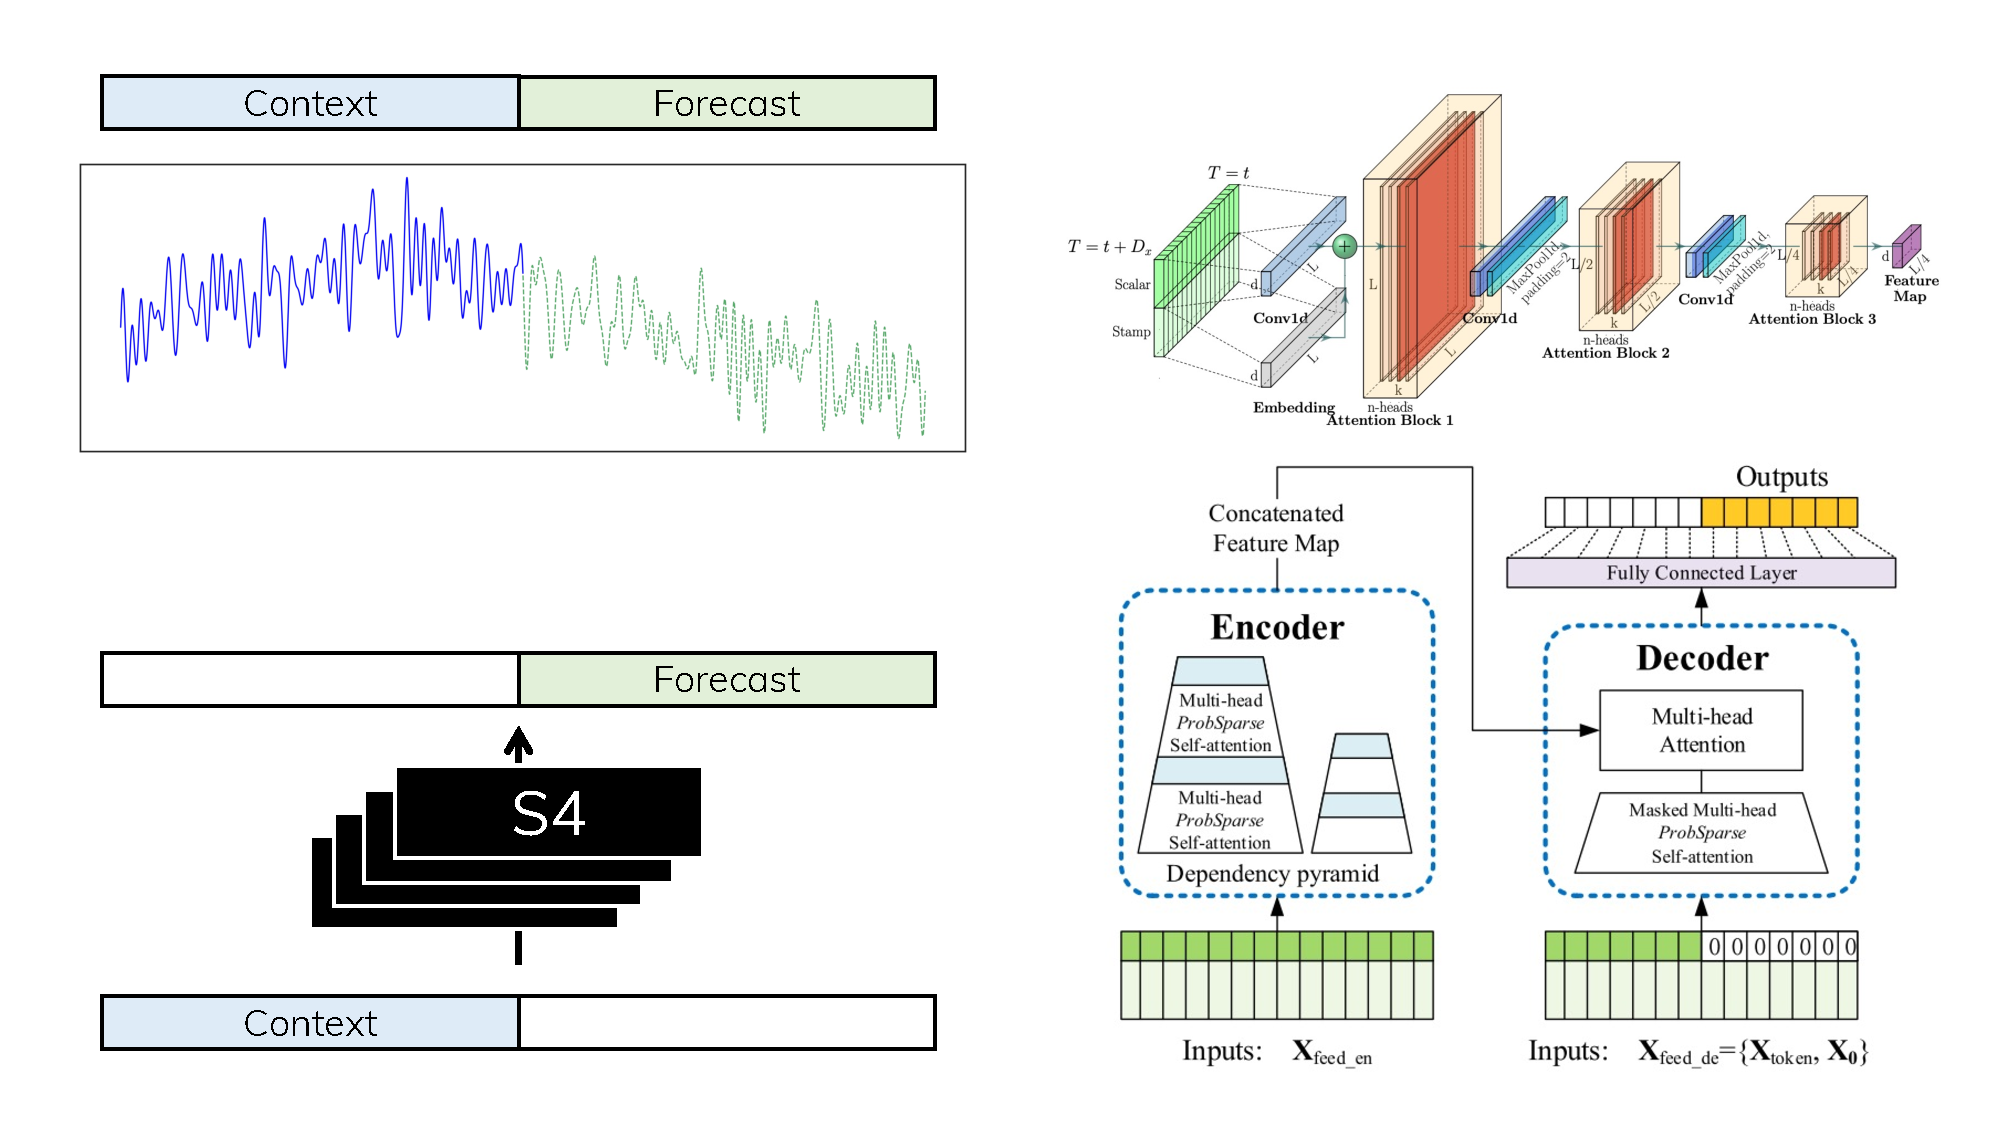
\includegraphics[width=\linewidth]{figs/s4_forecasting.pdf}
    \end{subfigure}
    \caption{Comparison of \methodabbrv{} and specialized time-series models for forecasting tasks. (\textit{Top Left}) The forecasting task involves predicting future values of a time-series given past context. (\textit{Bottom Left}) We perform simple forecasting using a sequence model such as \methodabbrv{} as a black box. (\textit{Right}) Informer uses an encoder-decoder architecture designed specifically for forecasting problems involving a customized attention module (figure taken from~\citet{haoyietal-informer-2021}).}
    \label{fig:s4-architecture}
\end{figure}

\cref{tab:informer-s,tab:informer-m} contain full results on all 50 settings considered by \citet{haoyietal-informer-2021}.
\methodabbrv{} sets the best results on 40 out of 50 of these settings.

\begin{table*}[t]
\centering
\fontsize{9pt}{9pt}\selectfont
\centering
\resizebox{\linewidth}{!}{
\begin{tabular}{c|c|c|c|c|c|c|c|c|c|c|c}
\toprule[1.0pt]
\multicolumn{2}{c|}{Methods}              & \textbf{\methodabbrv} & {Informer}                     & {Informer$^{\dag}$}            & {LogTrans}       & {Reformer}   & {LSTMa}      & {DeepAR}     & {ARIMA}                 & {Prophet}    \\
\midrule[0.5pt]
\multicolumn{2}{c|}{Metric}               & MSE~~MAE              & MSE~~MAE                       & MSE~~MAE                       & MSE~~MAE         & MSE~~MAE     & MSE~~MAE     & MSE~~MAE     & MSE~~MAE                & MSE~~MAE     \\
\midrule[1.0pt]
\multirow{5}{*}{\rotatebox{90}{ETTh$_1$}} & 24                    & \textbf{0.061}~~\textbf{0.191} & 0.098~~0.247                   & {0.092}~~{0.246} & 0.103~~0.259 & 0.222~~0.389 & 0.114~~0.272 & 0.107~~0.280            & 0.108~~0.284  & 0.115~~0.275 \\
                                          & 48                    & \textbf{0.079}~~\textbf{0.220} & {0.158}~~{0.319}               & 0.161~~0.322     & 0.167~~0.328 & 0.284~~0.445 & 0.193~~0.358 & 0.162~~0.327            & 0.175~~0.424  & 0.168~~0.330 \\
                                          & 168                   & \textbf{0.104}~~\textbf{0.258} & {0.183}~~{0.346}               & 0.187~~0.355     & 0.207~~0.375 & 1.522~~1.191 & 0.236~~0.392 & 0.239~~0.422            & 0.396~~0.504  & 1.224~~0.763 \\
                                          & 336                   & \textbf{0.080}~~\textbf{0.229} & 0.222~~0.387                   & {0.215}~~{0.369} & 0.230~~0.398 & 1.860~~1.124 & 0.590~~0.698 & 0.445~~0.552            & 0.468~~0.593  & 1.549~~1.820 \\
                                          & 720                   & \textbf{0.116}~~\textbf{0.271} & 0.269~~0.435                   & {0.257}~~{0.421} & 0.273~~0.463 & 2.112~~1.436 & 0.683~~0.768 & 0.658~~0.707            & 0.659~~0.766  & 2.735~~3.253 \\
\midrule[0.5pt]
\multirow{5}{*}{\rotatebox{90}{ETTh$_2$}} & 24                    & 0.095~~0.234                   & \textbf{0.093}~~\textbf{0.240} & 0.099~~0.241     & 0.102~~0.255 & 0.263~~0.437 & 0.155~~0.307 & 0.098~~0.263            & 3.554~~0.445  & 0.199~~0.381 \\
                                          & 48                    & 0.191~~0.346                   & \textbf{0.155}~~\textbf{0.314} & 0.159~~0.317     & 0.169~~0.348 & 0.458~~0.545 & 0.190~~0.348 & 0.163~~0.341            & 3.190~~0.474  & 0.304~~0.462 \\
                                          & 168                   & \textbf{0.167}~~\textbf{0.333} & {0.232}~~{0.389}               & 0.235~~0.390     & 0.246~~0.422 & 1.029~~0.879 & 0.385~~0.514 & 0.255~~0.414            & 2.800~~0.595  & 2.145~~1.068 \\
                                          & 336                   & \textbf{0.189}~~\textbf{0.361} & 0.263~~{0.417}                 & {0.258}~~0.423   & 0.267~~0.437 & 1.668~~1.228 & 0.558~~0.606 & 0.604~~0.607            & 2.753~~0.738  & 2.096~~2.543 \\
                                          & 720                   & \textbf{0.187}~~\textbf{0.358} & {0.277}~~{ 0.431}              & 0.285~~0.442     & 0.303~~0.493 & 2.030~~1.721 & 0.640~~0.681 & 0.429~~0.580            & 2.878~~1.044  & 3.355~~4.664 \\
\midrule[0.5pt]
\multirow{5}{*}{\rotatebox{90}{ETTm$_1$}} & 24                    & \textbf{0.024}~~\textbf{0.117} & {0.030}~~{0.137}               & 0.034~~0.160     & 0.065~~0.202 & 0.095~~0.228 & 0.121~~0.233 & 0.091~~0.243            & 0.090~~0.206  & 0.120~~0.290 \\
                                          & 48                    & \textbf{0.051}~~\textbf{0.174} & 0.069~~0.203                   & {0.066}~~{0.194} & 0.078~~0.220 & 0.249~~0.390 & 0.305~~0.411 & 0.219~~0.362            & 0.179~~0.306  & 0.133~~0.305 \\
                                          & 96                    & \textbf{0.086}~~\textbf{0.229} & 0.194~~{0.372}                 & {0.187}~~0.384   & 0.199~~0.386 & 0.920~~0.767 & 0.287~~0.420 & 0.364~~0.496            & 0.272~~0.399  & 0.194~~0.396 \\
                                          & 288                   & \textbf{0.160}~~\textbf{0.327} & {0.401}~~0.554                 & 0.409~~{0.548}   & 0.411~~0.572 & 1.108~~1.245 & 0.524~~0.584 & 0.948~~0.795            & 0.462~~0.558  & 0.452~~0.574 \\
                                          & 672                   & \textbf{0.292}~~\textbf{0.466} & {0.512}~~{0.644}               & 0.519~~0.665     & 0.598~~0.702 & 1.793~~1.528 & 1.064~~0.873 & 2.437~~1.352            & 0.639~~0.697  & 2.747~~1.174 \\
\midrule[0.5pt]
\multirow{5}{*}{\rotatebox{90}{Weather}}  & 24                    & 0.125~~0.254                   & \textbf{0.117}~~\textbf{0.251} & 0.119~~0.256     & 0.136~~0.279 & 0.231~~0.401 & 0.131~~0.254 & 0.128~~0.274            & 0.219~~0.355  & 0.302~~0.433 \\
                                          & 48                    & 0.181~~\textbf{0.305}          & \textbf{0.178}~~0.318          & 0.185~~0.316     & 0.206~~0.356 & 0.328~~0.423 & 0.190~~0.334 & 0.203~~0.353            & 0.273~~0.409  & 0.445~~0.536 \\
                                          & 168                   & \textbf{0.198}~~\textbf{0.333} & {0.266}~~{0.398}               & 0.269~~0.404     & 0.309~~0.439 & 0.654~~0.634 & 0.341~~0.448 & 0.293~~0.451            & 0.503~~0.599  & 2.441~~1.142 \\
                                          & 336                   & 0.300~~0.417                   & \textbf{0.297}~~\textbf{0.416} & 0.310~~0.422     & 0.359~~0.484 & 1.792~~1.093 & 0.456~~0.554 & 0.585~~0.644            & 0.728~~0.730  & 1.987~~2.468 \\
                                          & 720                   & \textbf{0.245}~~\textbf{0.375} & {0.359}~~{0.466}               & 0.361~~0.471     & 0.388~~0.499 & 2.087~~1.534 & 0.866~~0.809 & 0.499~~0.596            & 1.062~~0.943  & 3.859~~1.144 \\
\midrule[0.5pt]
\multirow{5}{*}{\rotatebox{90}{ECL}}      & 48                    & 0.222~~\textbf{0.350}          & 0.239~~0.359                   & 0.238~~0.368     & 0.280~~0.429 & 0.971~~0.884 & 0.493~~0.539 & \textbf{0.204}~~{0.357} & 0.879~~0.764  & 0.524~~0.595 \\
                                          & 168                   & 0.331~~\textbf{0.421}          & 0.447~~0.503                   & 0.442~~0.514     & 0.454~~0.529 & 1.671~~1.587 & 0.723~~0.655 & \textbf{0.315}~~{0.436} & 1.032~~0.833  & 2.725~~1.273 \\
                                          & 336                   & \textbf{0.328}~~\textbf{0.422} & 0.489~~0.528                   & 0.501~~0.552     & 0.514~~0.563 & 3.528~~2.196 & 1.212~~0.898 & {0.414}~~{0.519}        & 1.136~~0.876  & 2.246~~3.077 \\
                                          & 720                   & \textbf{0.428}~~\textbf{0.494} & {0.540}~~{0.571}               & 0.543~~0.578     & 0.558~~0.609 & 4.891~~4.047 & 1.511~~0.966 & 0.563~~0.595            & 1.251~~0.933  & 4.243~~1.415 \\
                                          & 960                   & \textbf{0.432}~~\textbf{0.497} & {0.582}~~{0.608}               & 0.594~~0.638     & 0.624~~0.645 & 7.019~~5.105 & 1.545~~1.006 & 0.657~~0.683            & 1.370~~0.982  & 6.901~~4.264 \\

\midrule[1.0pt]
\multicolumn{2}{c|}{Count}                & {22}                  & {5}                            & {0}                            & {0}              & {0}          & {0}          & {2}          & {0}                     & {0}          \\
\bottomrule[1.0pt]

\end{tabular}%
}
\caption{Univariate long sequence time-series forecasting results on four datasets (five cases).}
\label{tab:informer-s}
\end{table*}


\begin{table*}[t]
\centering
\fontsize{9pt}{9pt}\selectfont
\resizebox{\linewidth}{!}{
\begin{tabular}{c|c|cc|cc|cc|cc|cc|cc|cc}
\toprule[1.0pt]
\multicolumn{2}{c}{Methods}               & \multicolumn{2}{|c}{\textbf{\methodabbrv}} & \multicolumn{2}{|c}{Informer} & \multicolumn{2}{|c}{Informer$^{\dag}$} & \multicolumn{2}{|c}{LogTrans} & \multicolumn{2}{|c}{Reformer} & \multicolumn{2}{|c}{LSTMa} & \multicolumn{2}{|c}{LSTnet} \\
\midrule[0.5pt]
\multicolumn{2}{c|}{Metric}               & MSE                                        & MAE                           & MSE                                    & MAE                           & MSE                           & MAE                        & MSE                          & MAE     & MSE   & MAE   & MSE   & MAE   & MSE   & MAE     \\
\midrule[1.0pt]
\multirow{5}{*}{\rotatebox{90}{ETTh$_1$}} & 24                                         & \textbf{0.525}                & \textbf{0.542}                         & {0.577}                       & {0.549}                       & 0.620                      & 0.577                        & 0.686   & 0.604 & 0.991 & 0.754 & 0.650 & 0.624 & 1.293    & 0.901 \\
                                          & 48                                         & \textbf{0.641}                & \textbf{0.615}                         & {0.685}                       & {0.625}                       & 0.692                      & 0.671                        & 0.766   & 0.757 & 1.313 & 0.906 & 0.702 & 0.675 & 1.456    & 0.960 \\
                                          & 168                                        & 0.980                         & 0.779                                  & \textbf{0.931}                & \textbf{0.752}                & 0.947                      & 0.797                        & 1.002   & 0.846 & 1.824 & 1.138 & 1.212 & 0.867 & 1.997    & 1.214 \\
                                          & 336                                        & 1.407                         & 0.910                                  & 1.128                         & 0.873                         & \textbf{1.094}             & \textbf{0.813}               & 1.362   & 0.952 & 2.117 & 1.280 & 1.424 & 0.994 & 2.655    & 1.369 \\
                                          & 720                                        & \textbf{1.162}                & \textbf{0.842}                         & {1.215}                       & {0.896}                       & 1.241                      & 0.917                        & 1.397   & 1.291 & 2.415 & 1.520 & 1.960 & 1.322 & 2.143    & 1.380 \\
\midrule[0.5pt]
\multirow{5}{*}{\rotatebox{90}{ETTh$_2$}} & 24                                         & 0.871                         & 0.736                                  & \textbf{0.720}                & \textbf{0.665}                & 0.753                      & 0.727                        & 0.828   & 0.750 & 1.531 & 1.613 & 1.143 & 0.813 & 2.742    & 1.457 \\
                                          & 48                                         & \textbf{1.240}                & \textbf{0.867}                         & {1.457}                       & {1.001}                       & 1.461                      & 1.077                        & 1.806   & 1.034 & 1.871 & 1.735 & 1.671 & 1.221 & 3.567    & 1.687 \\
                                          & 168                                        & \textbf{2.580}                & \textbf{1.255}                         & 3.489                         & {1.515}                       & 3.485                      & 1.612                        & 4.070   & 1.681 & 4.660 & 1.846 & 4.117 & 1.674 & {3.242}  & 2.513 \\
                                          & 336                                        & \textbf{1.980}                & \textbf{1.128}                         & 2.723                         & 1.340                         & 2.626                      & {1.285}                      & 3.875   & 1.763 & 4.028 & 1.688 & 3.434 & 1.549 & {2.544}  & 2.591 \\
                                          & 720                                        & \textbf{2.650}                & \textbf{1.340}                         & {3.467}                       & {1.473}                       & 3.548                      & 1.495                        & 3.913   & 1.552 & 5.381 & 2.015 & 3.963 & 1.788 & 4.625    & 3.709 \\
\midrule[0.5pt]
\multirow{5}{*}{\rotatebox{90}{ETTm$_1$}} & 24                                         & 0.426                         & 0.487                                  & 0.323                         & \textbf{0.369}                & \textbf{0.306}             & 0.371                        & 0.419   & 0.412 & 0.724 & 0.607 & 0.621 & 0.629 & 1.968    & 1.170 \\
                                          & 48                                         & 0.580                         & 0.565                                  & 0.494                         & 0.503                         & \textbf{0.465}             & \textbf{0.470}               & 0.507   & 0.583 & 1.098 & 0.777 & 1.392 & 0.939 & 1.999    & 1.215 \\
                                          & 96                                         & 0.699                         & 0.649                                  & \textbf{0.678}                & 0.614                         & 0.681                      & \textbf{0.612}               & 0.768   & 0.792 & 1.433 & 0.945 & 1.339 & 0.913 & 2.762    & 1.542 \\
                                          & 288                                        & \textbf{0.824}                & \textbf{0.674}                         & {1.056}                       & {0.786}                       & 1.162                      & 0.879                        & 1.462   & 1.320 & 1.820 & 1.094 & 1.740 & 1.124 & 1.257    & 2.076 \\
                                          & 672                                        & \textbf{0.846}                & \textbf{0.709}                         & {1.192}                       & {0.926}                       & 1.231                      & 1.103                        & 1.669   & 1.461 & 2.187 & 1.232 & 2.736 & 1.555 & 1.917    & 2.941 \\
\midrule[0.5pt]
\multirow{5}{*}{\rotatebox{90}{Weather}}  & 24                                         & \textbf{0.334}                & 0.385                                  & {0.335}                       & \textbf{0.381}                & 0.349                      & 0.397                        & 0.435   & 0.477 & 0.655 & 0.583 & 0.546 & 0.570 & 0.615    & 0.545 \\
                                          & 48                                         & 0.406                         & 0.444                                  & 0.395                         & 0.459                         & \textbf{0.386}             & \textbf{0.433}               & 0.426   & 0.495 & 0.729 & 0.666 & 0.829 & 0.677 & 0.660    & 0.589 \\
                                          & 168                                        & \textbf{0.525}                & \textbf{0.527}                         & {0.608}                       & {0.567}                       & 0.613                      & 0.582                        & 0.727   & 0.671 & 1.318 & 0.855 & 1.038 & 0.835 & 0.748    & 0.647 \\
                                          & 336                                        & \textbf{0.531}                & \textbf{0.539}                         & {0.702}                       & {0.620}                       & 0.707                      & 0.634                        & 0.754   & 0.670 & 1.930 & 1.167 & 1.657 & 1.059 & 0.782    & 0.683 \\
                                          & 720                                        & \textbf{0.578}                & \textbf{0.578}                         & {0.831}                       & {0.731}                       & 0.834                      & 0.741                        & 0.885   & 0.773 & 2.726 & 1.575 & 1.536 & 1.109 & 0.851    & 0.757 \\
\midrule[0.5pt]
\multirow{5}{*}{\rotatebox{90}{ECL}}      & 48                                         & \textbf{0.255}                & \textbf{0.352}                         & 0.344                         & {0.393}                       & 0.334                      & 0.399                        & 0.355   & 0.418 & 1.404 & 0.999 & 0.486 & 0.572 & 0.369    & 0.445 \\
                                          & 168                                        & \textbf{0.283}                & \textbf{0.373}                         & 0.368                         & 0.424                         & {0.353}                    & {0.420}                      & 0.368   & 0.432 & 1.515 & 1.069 & 0.574 & 0.602 & 0.394    & 0.476 \\
                                          & 336                                        & \textbf{0.292}                & \textbf{0.382}                         & 0.381                         & {0.431}                       & 0.381                      & 0.439                        & {0.373} & 0.439 & 1.601 & 1.104 & 0.886 & 0.795 & 0.419    & 0.477 \\
                                          & 720                                        & \textbf{0.289}                & \textbf{0.377}                         & 0.406                         & 0.443                         & {0.391}                    & {0.438}                      & 0.409   & 0.454 & 2.009 & 1.170 & 1.676 & 1.095 & 0.556    & 0.565 \\
                                          & 960                                        & \textbf{0.299}                & \textbf{0.387}                         & {0.460}                       & {0.548}                       & 0.492                      & 0.550                        & 0.477   & 0.589 & 2.141 & 1.387 & 1.591 & 1.128 & 0.605    & 0.599 \\
\midrule[1.0pt]
\multicolumn{2}{c}{Count}                 & \multicolumn{2}{|c}{18}                    & \multicolumn{2}{|c}{5}        & \multicolumn{2}{|c}{6}                 & \multicolumn{2}{|c}{0}        & \multicolumn{2}{|c}{0}        & \multicolumn{2}{|c}{0}     & \multicolumn{2}{|c}{0}      \\
\bottomrule[1.0pt]

\end{tabular}%
}
\caption{Multivariate long sequence time-series forecasting results on four datasets (five cases).}
\label{tab:informer-m}
\end{table*}


\subsection{Visualizations}
We visualize the convolutional filter $\bar{K}$ learned by \methodabbrv{} for the Pathfinder and CIFAR-10 tasks in \cref{fig:pathfinder-all-conv-filters}.

\begin{figure}
    \centering
    \begin{subfigure}{\linewidth}
        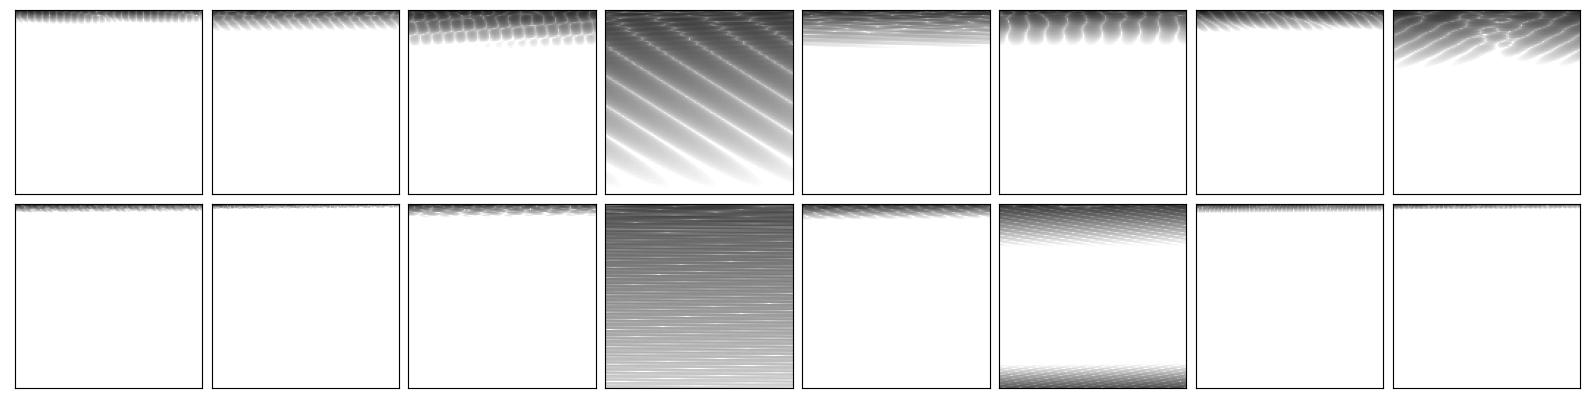
\includegraphics[width=\linewidth]{figs/pathfinder_filters_layer_0_trunc.png}
    \end{subfigure}
    \begin{subfigure}{\linewidth}
        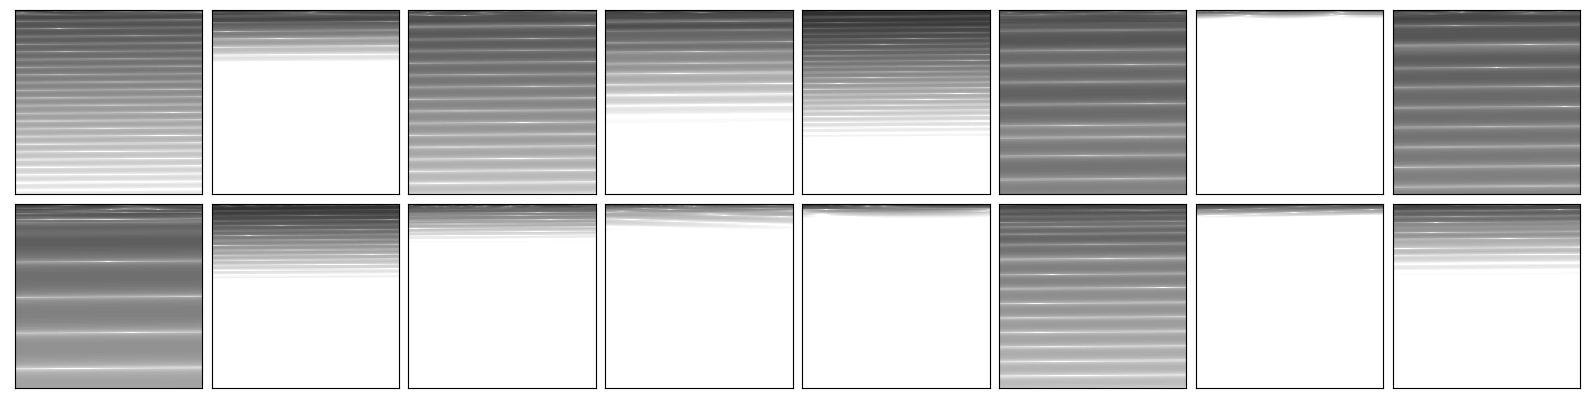
\includegraphics[width=\linewidth]{figs/pathfinder_filters_layer_5_trunc.png}
    \end{subfigure}
    \label{fig:pathfinder-all-conv-filters}
    \caption{({\bf Convolutional filters on Pathfinder}) A random selection of filters learned by \methodabbrv{} in the first layer (top 2 rows) and last layer (bottom 2 rows) of the best model.}
\end{figure}

\subsection{Reproduction}
\label{sec:reproduction}

Since the first version of this paper, several experiments have been updated. Please read the corresponding paragraph below before citing LRA or SC results.

\paragraph{Long Range Arena}

Follow-ups to this paper expanded the theoretical understanding of S4 while improving some results.
The results reported in \cref{tab:lra} have been updated to results from the papers \citep{gu2022s4d,gu2022hippo}.
More specifically, the method S4-LegS in those works refers to the \emph{same model} presented in this paper, with the ``-LegS'' suffix referring to the initialization defined in equation \eqref{eq:hippo}. As such, results from the original \cref{tab:lra} have been directly updated.

The updated results have only minor hyperparameter changes compared to the original results. The original results and hyperparameters are shown in \cref{tab:lra-full} (\cref{sec:experiment-details-lrd}).
Appendix B of \citep{gu2022s4d} describes the changes in hyperparameters, which are also documented from the experiment configuration files in the publically available code at \url{https://github.com/HazyResearch/state-spaces}.

\paragraph{Speech Commands}

The Speech Commands (SC) dataset~\citep{Warden2018SpeechCA} is originally a 35-class dataset of spoken English words.
However, this paper was part of a line of work starting with \citet{kidger2020neural} that has used a smaller 10-class subset of SC \citep{kidger2020neural,romero2021ckconv,gu2021lssl,romero2022flexconv}.
\emph{In an effort to avoid dataset fragmentation in the literature, we have since moved to the original dataset.}
We are now calling this 10-class subset \textbf{SC10} to distinguish it from the full 35-class \textbf{SC} dataset.
To cite S4 as a baseline for Speech Commands, please use Table 11 from \citep{gu2022s4d} instead of \cref{tab:sc} from this paper.
In addition to using the full SC dataset, it also provides a number of much stronger baselines than the ones used in this work.


\paragraph{WikiText-103}

The original version of this paper used an S4 model with batch size \( 8 \), context size \( 1024 \) which achieved a validation perplexity of 20.88 and test perplexity of 21.28.
It was later retrained with a batch size of \( 1 \) and context size \( 8192 \) which achieved a validation perplexity of 19.69 and test perplexity of 20.95, and a model checkpoint is available in the public repository.
The rest of the model is essentially identical, so the results from the original table have been updated.
